\documentclass[../../../main]{subfiles}
\begin{document}

\section{結果}

\subsection{実験1}
MTJ素子に磁場をかけていない状態で電流\SI{12.40}{\micro A}を与えたときの電圧は\SI{21.4518}{mA}であった。
これよりMTJ素子の抵抗値は$R = \SI{1.746}{k\ohm}$である。

\subsection{実験2, 3}
実験2, 3の結果を表\ref{tab:7to-7}と表\ref{tab:-7to7}に示す。
また、この表からTMR比を求めると、\SI{153.5}{\%}となった。
さらに、磁場と$H$とMTJ素子の抵抗$R$の関係を図示すると、図\ref{fig:result}のようになる。

\begin{table}[!ht]
	\centering
	\caption{磁場による抵抗値の変化(\SI{7}{A}から\SI{-7}{A}まで変化させたとき)}
	\label{tab:7to-7}
	\begin{tabular}{cccccc}
		\hline
		セット電流 / A & 磁場 / mT & 実測電流 / A & 電流 / \si{\micro A} & 電圧 / \si{\micro V} & 抵抗 / \si{\ohm} \\ \hline
		7         & 109.1   & 11.038   & 12.43              & 17892.8            & 1439           \\
		6         & 94.4    & 9.4811   & 12.42              & 18517.3            & 1490           \\
		5         & 79.2    & 7.9211   & 12.41              & 19478.2            & 1569           \\
		4         & 63.8    & 6.364    & 12.40              & 21153.0            & 1705           \\
		3         & 48.4    & 4.8039   & 12.37              & 25577.6            & 2067           \\
		2.5       & 40.7    & 4.0239   & 12.34              & 29305.1            & 2374           \\
		2         & 32.9    & 3.2438   & 12.30              & 33726.9            & 2742           \\
		1.5       & 25.4    & 2.4638   & 12.28              & 36795.7            & 2996           \\
		1         & 17.1    & 1.6822   & 12.26              & 38641.7            & 3151           \\
		0.75      & 12.8    & 1.293    & 12.26              & 39152.1            & 3193           \\
		0.5       & 9.2     & 0.9037   & 12.26              & 39620.0            & 3231           \\
		0.25      & 5.4     & 0.5129   & 12.26              & 39209.1            & 3198           \\
		0.125     & 3.3     & 0.3183   & 12.27              & 37847.1            & 3084           \\
		0         & 1.4     & 0.1222   & 12.32              & 30967.4            & 2513           \\
		-0.125    & -0.4    & -0.0753  & 12.40              & 20634.1            & 1664           \\
		-0.25     & -2.4    & -0.2699  & 12.43              & 17346.3            & 1395           \\
		-0.5      & -6.2    & -0.6574  & 12.44              & 16480.4            & 1324           \\
		-0.75     & -10.1   & -1.0494  & 12.44              & 16407.9            & 1318           \\
		-1        & -14.1   & -1.44    & 12.44              & 16374.8            & 1316           \\
		-1.5      & -21.9   & -2.2196  & 12.44              & 16339.6            & 1313           \\
		-2        & -29.7   & -2.9976  & 12.44              & 16314.4            & 1311           \\
		-2.5      & -37.5   & -3.7802  & 12.44              & 16297.4            & 1310           \\
		-3        & -45.2   & -4.5568  & 12.44              & 16278.1            & 1308           \\
		-4        & -60.8   & -6.119   & 12.44              & 16272.1            & 1308           \\
		-5        & -70.5   & -7.6781  & 12.44              & 16265.8            & 1307           \\
		-6        & -92.1   & -9.2373  & 12.44              & 16262.2            & 1307           \\
		-7        & -107.6  & -10.797  & 12.44              & 16265.0            & 1307           \\ \hline
	\end{tabular}
\end{table}

\begin{table}[!ht]
	\centering
	\caption{磁場による抵抗値の変化(\SI{-7}{A}から\SI{7}{A}まで変化させたとき)}
	\label{tab:-7to7}
	\begin{tabular}{cccccc}
		\hline
		セット電流 / A & 磁場 / mT & 実測電流 / A & 電流 / \si{\micro A} & 抵抗 / \si{mV} & 抵抗 / \Omega \\ \hline
		7         & 109.3   & 11.038   & 12.40              & 17.9900      & 1450        \\
		6         & 93.1    & 9.4796   & 12.40              & 19.2372      & 1551        \\
		5         & 78.1    & 7.9196   & 12.40              & 21.2915      & 1717        \\
		4         & 62.7    & 6.3625   & 12.37              & 24.4237      & 1974        \\
		3         & 46.7    & 4.8024   & 12.32              & 31.5320      & 2559        \\
		2.5       & 38.8    & 4.0224   & 12.28              & 32.5231      & 2648        \\
		2         & 31      & 3.2438   & 12.26              & 38.1000      & 3107        \\
		1.5       & 23.3    & 2.4623   & 12.25              & 39.5640      & 3229        \\
		1         & 15.3    & 1.6822   & 12.25              & 40.3951      & 3297        \\
		0.75      & 11.3    & 1.2915   & 12.25              & 40.5889      & 3313        \\
		0.5       & 7.4     & 0.9022   & 12.25              & 40.4031      & 3298        \\
		0.25      & 3.4     & 0.5129   & 12.29              & 35.4221      & 2882        \\
		0.125     & 1.6     & 0.3138   & 12.36              & 25.7968      & 2087        \\
		0         & 1.5     & 0.1237   & 12.42              & 18.5730      & 1495        \\
		-0.125    & -2.5    & -0.0723  & 12.43              & 16.8467      & 1355        \\
		-0.25     & -4.4    & -0.2699  & 12.43              & 16.5220      & 1329        \\
		-0.5      & -8.3    & -0.6574  & 12.43              & 16.4082      & 1320        \\
		-0.75     & -12.2   & -1.0494  & 12.43              & 16.3747      & 1317        \\
		-1        & -16.1   & -1.4400  & 12.44              & 16.3555      & 1314        \\
		-1.5      & -23.9   & -2.2196  & 12.44              & 16.3303      & 1312        \\
		-2        & -31.7   & -2.9991  & 12.44              & 16.3127      & 1311        \\
		-2.5      & -38.8   & -3.7802  & 12.44              & 16.2992      & 1310        \\
		-3        & -47.1   & -4.5583  & 12.44              & 16.2893      & 1309        \\
		-4        & -62.5   & -6.1190  & 12.44              & 16.2753      & 1308        \\
		-5        & -77.7   & -7.6796  & 12.44              & 16.2682      & 1307        \\
		-6        & -92.9   & -9.2373  & 12.44              & 16.2651      & 1307        \\
		-7        & -108    & -10.797  & 12.44              & 16.2661      & 1307        \\ \hline
	\end{tabular}
\end{table}

\begin{figure}
	\centering
	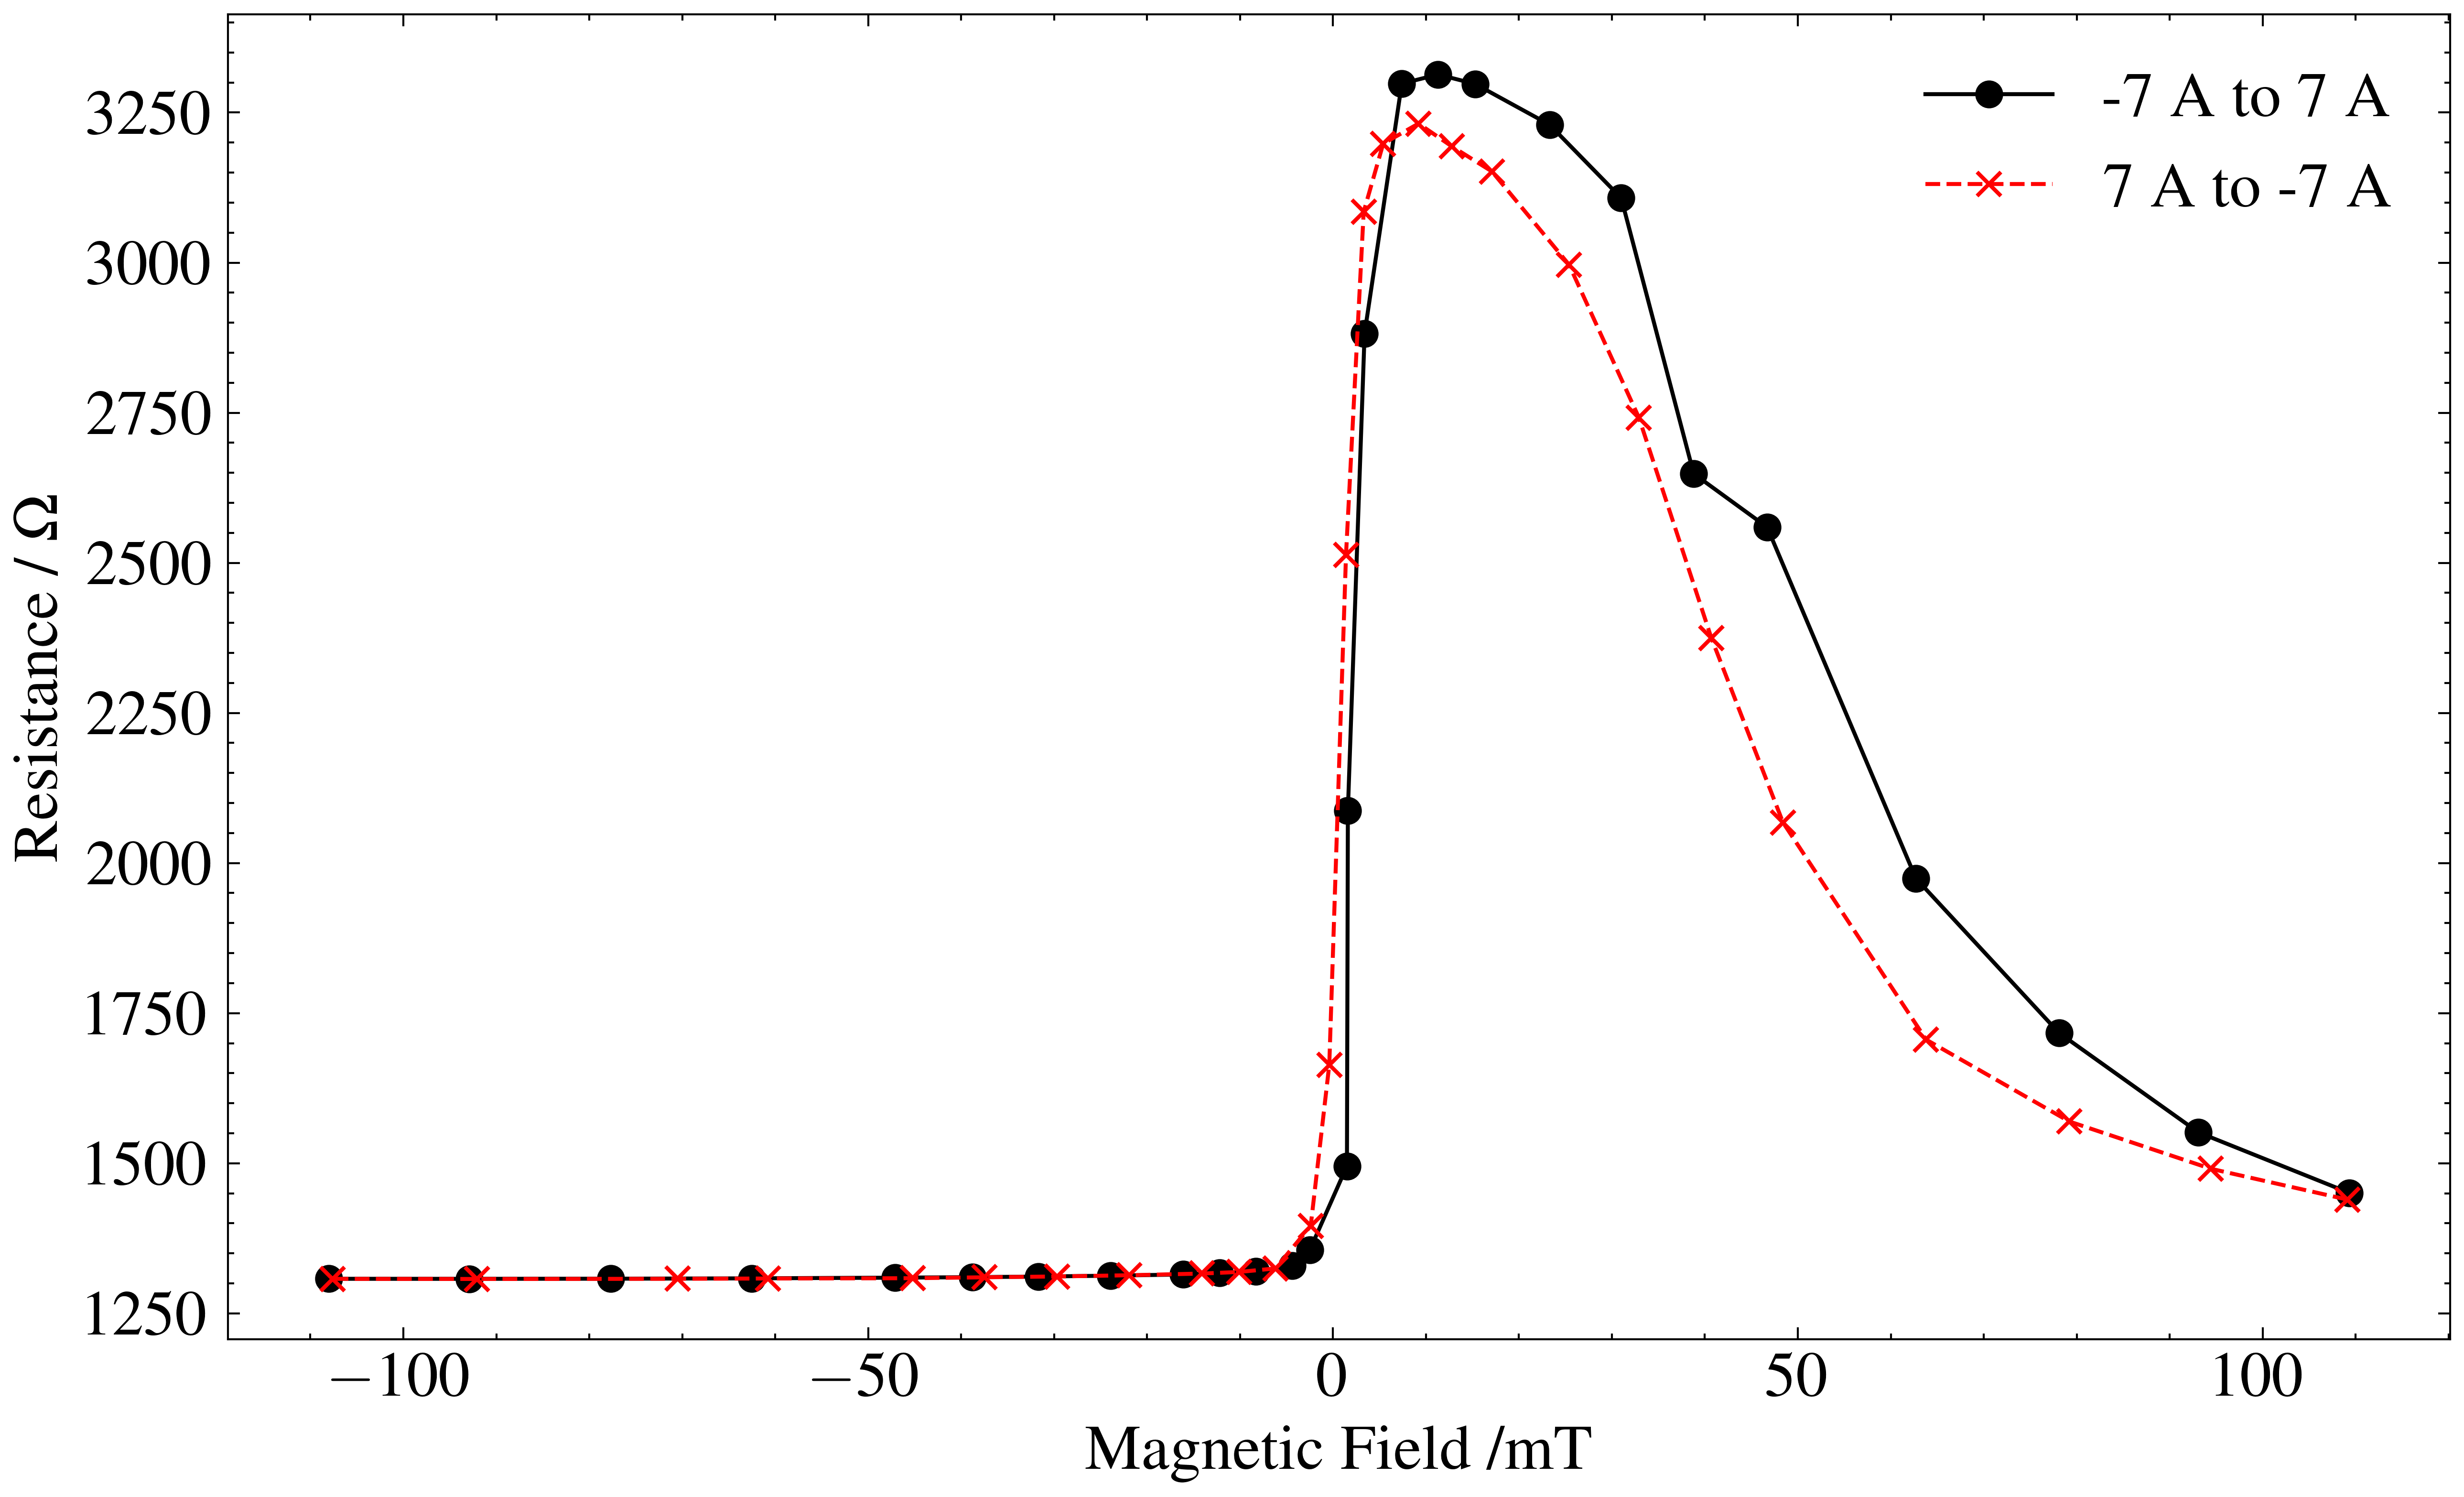
\includegraphics[width=0.8\linewidth]{src/figures/result/result.png}
	\caption{磁場$H$とそのときのMTJの抵抗値の関係}\label{fig:result}
\end{figure}


\end{document}
